\documentclass[../main.tex]{subfiles}

\begin{document}

\renewcommand{\labelitemi}{\ding{226}}
\renewcommand{\labelitemii}{\ding{227}}

\chapter{The T2K experiment}
\label{ch:T2K:general}

The T2K (Tokai to Kamioka) is a long-baseline accelerator neutrino experiment. Its main purpose is precise measurements of the neutrino oscillation parameters. T2K is a continuation of the successful history of the previous accelerator experiments: KEK, MINOS, etc. At the beginning of the T2K era, the main challenge was the measurements of the $\theta_{13}$ mixing angle. Only the upper limit on its value was set at that moment and $\theta_{13}=0$ was possible. The value of this angle is important as the amplitude of the CP--violation (\autoref{sec:intro:cp} of \autoref{ch:nu_phys}) is scaled with $\theta_{13}$ angle. If $\theta_{13}$ is equal to zero no CP--violation effect can be observed. Thus $\theta_{13}$ angle measurements became the main goal at the beginning of the T2K era.

The $\theta_{13}$ angle can be measured in both appearance ($\nu_\alpha\to\nu_\beta$) and disappearance ($\nu_\alpha\to\nu_\alpha$) channels. The reactor experiments are very powerful in the analysis of the $\overline{\nu}_e\to\overline{\nu}_e$ disappearance process and thus can measure $\theta_{13}$ angle precisely. But the CP--violation effect can take place only in the appearance channel (\autoref{sec:intro:cp} of \autoref{ch:nu_phys}). The $\nu_e\to\nu_\mu$ channel is extremely challenging from the experimental point of view. There is no easy way to create an intense pure beam of high energetic electron neutrinos. On the contrary, the $\nu_\mu\to\nu_e$ channel is very promising. The charged mesons (e.g. pions, kaons) decay mainly into the muon neutrino. And the intense and focused beam of charged mesons can be easily created with a particle accelerator. Thus the accelerator experiments are the only way to probe the CP--violation. Also, they are very powerful in the measurements of the $\theta_{13}$, $\theta_{23}$ and $\Delta m^2_{32}$ parameters.

The approach of the accelerator oscillation experiment is to measure the energy spectrum of the neutrino beam at the far detector and compare it to the expectations without the oscillations. The reconstruction of the energy is critical as neutrino oscillates along $L/E_\nu$. While the baseline $L$ is fixed neutrino with different energies will arrive at the far detector in the different phase of the oscillation. The expected neutrino flux can be constrained with the measurements of the unoscillated neutrinos with the near detector. In the T2K the neutrino energy is reconstructed with the water Cherenkov detector Super--Kamiokande (\autoref{sec:T2K:sk}) and the magnetized near detector ND280 (\autoref{sec:T2K:nd280}). The water detector measures the energy of the particle with the opening angle of Cherenkov radiation and the ND280 measures the momentum with the track curvature in the magnetic field. The easiest way to measure neutrino energy is to work in the energy region where the most probable neutrino interaction is quasi-elastic $\nu_\ell+n\to\ell^-+p$ ($\overline{\nu}_\ell+p\to\ell^++n$). As this is a two-body process and the incoming neutrino direction is known the neutrino energy can be calculated with the outgoing lepton kinematics only. This reaction dominates at energies below 1 GeV. But if the neutrino has higher energy then several particles can be produced. Some of them can be low energetic or neutral hence will not be detected. That makes the neutrino energy reconstruction extremely difficult. The problem is that the mesons with the wide energy range are produced in the proton beam interactions in the target. That results in a very wide neutrino spectrum. To deal with this T2K uses the ``off-axis'' beam to produce quasi-monoenergetic neutrino flux (\autoref{sec:T2K:oa_flux}).

T2K was designed to measure the appearance process $\overset{\scriptscriptstyle(-)}{\nu}_\mu\to\overset{\scriptscriptstyle(-)}{\nu}_e$ which was expected to be rather rare. First of all the signal rate should be enhanced as much as possible. The J-PARC accelerator provides a very intense muon neutrino beam. Further improvement is considered (\autoref{sec:up:beam} of \autoref{ch:up:motif}). Secondly, all the processes that can mimic the $\nu_\mu\to\nu_e$ signal should be suppressed or precisely controlled. One of the main concerns is the electron neutrinos initially produced in the beamline. The meson's decay mostly leads to the muon and muon neutrino production. But the muon decay will result in the electron anti-neutrino $\mu^-\to e^-\overline{\nu}_e\nu_\mu$. To suppress such a process, the length of the meson decay volume is limited. The produced muons are stopped in the beam dump just after the decay pipe and emit the electron neutrinos isotropically, not pointed towards the far detector. The second process of concern is the neutral pion production in the neutrino interactions through the neutral current. The $\pi^0$ will further decay into two photons. At our energies, photons will convert into the electron-positron pair. In the case of asymmetric $\pi^0$ decay, one of the components of the pair can be lost resulting in the detection of a single electromagnetic shower. The SK doesn't distinguish electrons and positrons thus $NC\pi^0$ event can mimic the electron production from the neutrino interaction. To estimate the rate of the neutral pion production the special $\pi^0$ subdetector was built in the near detector complex (\autoref{sec:t2k:pod}).

When studying the CP--violation it is critical to distinguish neutrino and anti-neutrino oscillations since the effect is the opposite for them. The Super---Kamiokande can not separate $\mu^+$ from $\mu^-$ (electrons from positrons) as Cherenkov rings will be similar for them. Thus the neutrino can not be distinguished from the anti-neutrino. The near detector ND280 is magnetized. Charged current neutrino and anti-neutrino interactions will produce leptons of the opposite charge. Their tracks will curve in opposite directions and can be easily separated. Therefore the contamination of the anti-neutrino in the neutrino beam and vice-versa can be measured. The effect of the wrongly reconstructed neutrino type can be taken into account in the oscillation analysis. Hence the CP--violation is measured much more precisely with this additional information.

The sketch of the T2K setup is shown in \autoref{fig:t2k:t2k_scheme}. In brief, the overall scheme of the T2K experiment is the following:
\begin{enumerate}
  \item The proton beam hits the carbon target producing mesons.
  \item The mesons are focused with horns into the decay volume. The horn polarity defines whether positively or negatively charged mesons will be focused.
  \item In the decay volume, the mesons decay mostly into the muon neutrino or anti-neutrino. Thus the horn polarity defines the neutrino mode: ($H^+\to\mu^+\nu_{\mu}$ or $H^-\to\mu^-\overline{\nu}_{\mu}$). The energy spectrum of the off-axis neutrino beam is quasi-monoenergetic peaking around 0.6 GeV.
  \item The muons from the meson decays are mostly stopped in the beam dump, preventing the large electron neutrino contribution in the flux.
  \item The neutrino beam intensity and direction are constantly monitored by the muon monitor and the on-axis detector INGRID.
  \item The neutrino and anti-neutrino fraction, the neutrino flavor and energy spectrum of the non-oscillated beam is measured with the off-axis ND280 detector (\autoref{sec:T2K:nd})
  \item After traveling 295 km the neutrino beam reaches the far detector complex Super-Kamiokande (\autoref{sec:T2K:sk}). The baseline and neutrino energy are fixed at the first oscillation maximum ($\Delta m ^2_{32}L/E\approx1$).
\end{enumerate}

\begin{figure}[!ht]
  \centering
  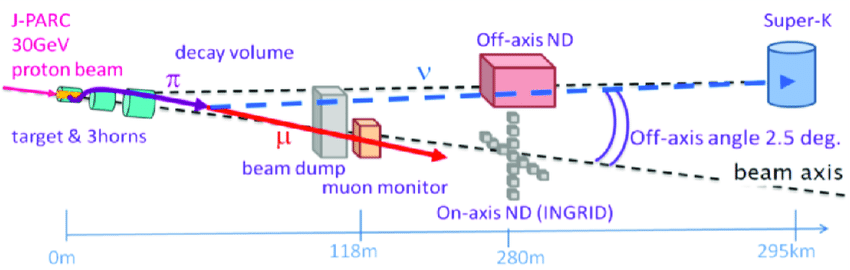
\includegraphics[width=0.95\linewidth]{t2k_scheme}
  \caption{The sketch of the T2K setup shows all the key elements of the experiment.}
  \label{fig:t2k:t2k_scheme}
\end{figure}

The main goals of the T2K experiment are:
\begin{itemize}
  \item precise measurements of the oscillation parameters $\Delta m^2_{23}$ and $\theta_{23}$ with the muon (anti--) neutrino disappearance $\nu_\mu\to\nu_\mu$ ($\overline{\nu}_\mu\to\overline{\nu}_\mu$)
  \item measurements of the  $\theta_{13}$ angle with the electron appearance $\nu_\mu\to\nu_e$ and $\overline{\nu}_\mu\to\overline{\nu}_e$
  \item search for the CP violation $\sin\delta_{CP}\neq0$ by studying the difference between $\nu_\mu\to\nu_e$ and $\overline{\nu}_\mu\to\overline{\nu}_e$
  \item along with the oscillation measurements, the neutrino interactions are studied carefully to reduce the systematic uncertainty. Thus the neutrino cross-sections on carbon, water and iron are measured.
\end{itemize}

T2K successfully measured the non-zero value of the $\theta_{13}$~\cite{Abe2014a, An2012} and made a discovery detecting $\nu_\mu\to\nu_e$ appearance thus opening the way for the CP--violation search. At the moment it is a major goal of the experiment together with more precise measurements of other oscillation parameters. In this chapter, the details about the T2K setup as well as an analysis technique will be overviewed.

\section{Neutrino beam}
\label{ch:T2K:nu_beam}

The proton accelerator is used for the production of the T2K neutrino beam. The 30 GeV kinetic energy protons from the J-PARC accelerator hit the target producing mesons. At these energies mainly pions are produced. There is still some minor contribution of kaons in the meson flux. Mesons with the proper charge are focused in the decay volume while the wrong-charged mesons are defocused and neutral particles remain unfocused. In the decay volume, the mesons decay mainly into the muon and muon neutrino. The decay to the electron and electron neutrino is suppressed by 4 orders by the V-A structure of the weak interaction. The mesons of the same charge always produce neutrino or anti-neutrino. Thus the wrong-sign component of the neutrino beam is severely suppressed with the meson focusing system. The polarity of the focusing system may be changed resulting in an almost pure neutrino or anti-neutrino beam.

The accelerator neutrino experiment has several benefits as it uses a man-made neutrino beam. It is focused, thus extremely intense, high energetic and precisely controlled. It mostly consists of muon neutrino. The possibility to switch between neutrinos or anti-neutrinos beam is critical for the CP--violation search. To constrain the $\delta_{CP}$ phase the difference between neutrino and anti-neutrino oscillations should be studied. The beam monitoring reduces the systematic uncertainties related to the flux. The intense pure beam of the muon neutrino is essential for the precise studies of the $\nu_\mu\to\nu_e$ oscillations. The purity of the beam will minimize the electron neutrino contamination in the neutrino beam that is a background for the $\nu_e$ appearance process. The lower background will make easier the signal observation. In this section, the details about the beam production and monitoring within the T2K experiment will be presented.

\subsection{Off-axis flux}
\label{sec:T2K:oa_flux}
Mesons produced in the proton collisions have a wide energy spectrum. That leads to a wide range of neutrino energies. It makes the oscillation analysis difficult. Neutrino oscillation depends on $L/E_\nu$. Thus for the given baseline, only neutrinos with the given energy will demonstrate the maximum appearance or disappearance. All the neutrinos with other energies will be less affected by the oscillations and can mask the process of interest. As mentioned in the introduction, to gain energy reconstruction precision only quasi-elastic interactions are used. It means that we are looking for events with one lepton and nothing more. The incoming neutrino energy is estimated assuming the quasi-elastic interaction as well. This is a dominant topology of the neutrino interactions at the energies below 1 GeV. With energy growth, the cross-section of the neutrino interactions dramatically increases. The main reaction becomes deep inelastic processes with a production of several different particles. If the particle energy is lower then the threshold of Cherenkov radiation emission it is completely invisible in the Super--Kamiokande. Thus high energy neutrinos are a very nuisance for the T2K. They interact more often and produce many particles that can be low energetic. Hence we can wrongly classify such an event as quasi-elastic and reconstruct the neutrino energy with the wrong assumption.

To handle this the T2K experiment uses a so-called ``off-axis'' concept to obtain a quasi-monoenergetic neutrino beam. The key idea is to use not the neutrinos pointed along the beam axis, but directed at a slight angle. Such neutrinos will have a relatively narrow energy spectrum. The dominating neutrino production mode in the T2K is a pion decay $\pi\to\mu\nu$. The neutrino energy in the two-body decay in the laboratory frame will be given by
\begin{equation}
E_\nu\approx\left(1-\frac{m_\mu^2}{m_\pi^2}\right)\frac{E_\pi}{1+\gamma^2\theta^2}
\end{equation}

where $\gamma$ is the pion kinematic parameter and $\theta$ is a neutrino direction angle w.r.t. pion momentum. The equality of the derivative of the neutrino energy over the pion energy to zero means full independence of the first from the latter. In case $\theta=\gamma^{-1}$, the derivative of the neutrino energy becomes zero $dE_\nu/dE_\pi=0$ that means that the energy depends weakly on the parent pion momentum. Finally, we will get
\begin{equation}
E_\nu\approx\left(1-\frac{m_\mu^2}{m_\pi^2}\right)\frac{m_\pi}{2\theta}\approx\frac{29.8MeV}{\theta\left[rad\right]}
\end{equation}

The T2K beamline was set to the 2.5${}^\circ$ off-axis angle. It was tuned to set the neutrino energy peak to the oscillation maximum. With the fixed mixing angle and mass difference the energy spectra for different angles are shown in \autoref{fig:t2k:nu_beam_oa}. The figure provides also the oscillation probability of the muon neutrino at a distance of 295 km versus the energy. Thus with the off-axis angle tuning the maximum oscillation effect can be measured. Though the high energy neutrinos are harmful to the oscillation analysis nevertheless high energy mesons can be useful for other studies. For example, they can be helpful for the Heavy Neutral Lepton (HNL \autoref{sec:intro:HNL}) search. High energy mesons decay will result in the focused HNL beam while low energy mesons will produce HNL over a very wide angle. The heavy neutrino study is one of the main topics of the current thesis (\autoref{ch:hnl}).

\begin{figure}[!ht]
  \centering
  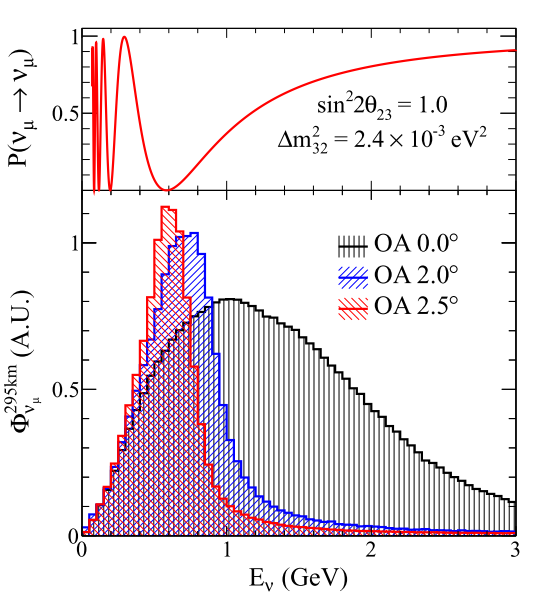
\includegraphics[width=0.5\linewidth]{nu_beam}
  \caption{Muon neutrino survival probability at 295 km and neutrino fluxes for different off-axis angles. Figure from~\cite{Abe2013}.}
  \label{fig:t2k:nu_beam_oa}
\end{figure}

\subsection{Neutrino beamline}
The T2K neutrino beamline can be generally divided into two stages: primary beamline and secondary beamline. The first takes the protons from the J-PARC accelerator main ring, performs measurements of the beam parameters and focuses it on a carbon target. The secondary beamline focuses the produced mesons with the horns into the decay volume and monitors its decay. The general scheme of the beamline is shown in \autoref{fig:t2k:beamline}. A detailed description can be found in~\cite{Abe2013}.

\begin{figure}[!ht]
  \centering
  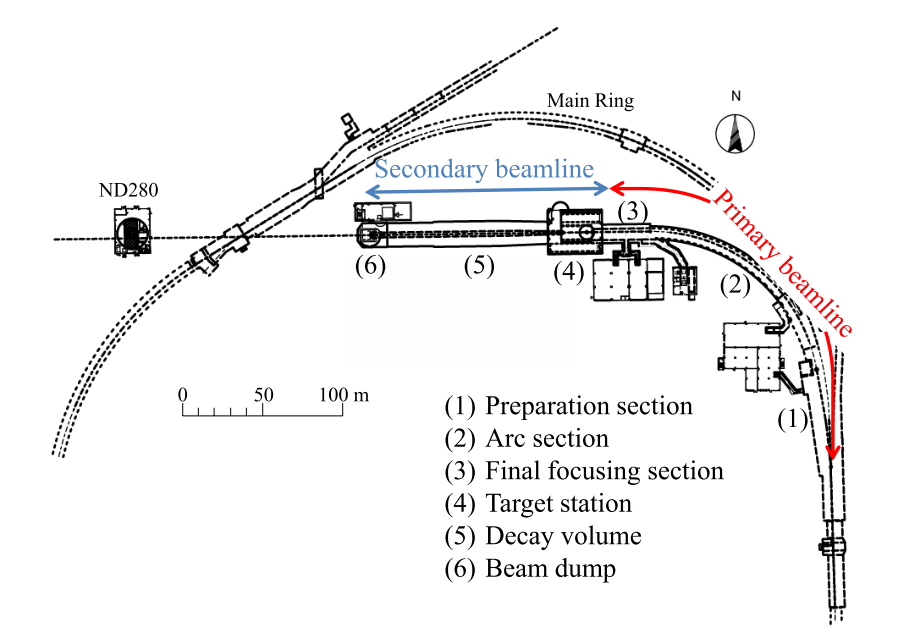
\includegraphics[width=0.7\linewidth]{beamline}
  \caption{The scheme of the T2K neutrino beam line. Primary beamline (proton line) is shown in red and secondary beamline is shown in blue.}
  \label{fig:t2k:beamline}
\end{figure}

\subsubsection{Primary beamline}
The primary beamline takes the proton from the J-PARC main ring. The beam is structured into the spills coming with 0.5 Hz rate. Each spill is 5 $\mu\text{s}$ wide and consists of 8 bunches with $\sigma\approx18 \text{ ns}$ and 58 ns separation. Per each spill, $3\times10^{14}$ protons can be delivered. Thus the total maximum power of the beamline can be estimated as 750 kW. The total number of protons hitting the target (POT - Protons On Target) is used as the main measure of the statistics collected in the T2K experiment. The evolution of the accumulated statistics, as well as the beam power, is shown in \autoref{fig:t2k:POT}.

\begin{figure}[!ht]
  \centering
  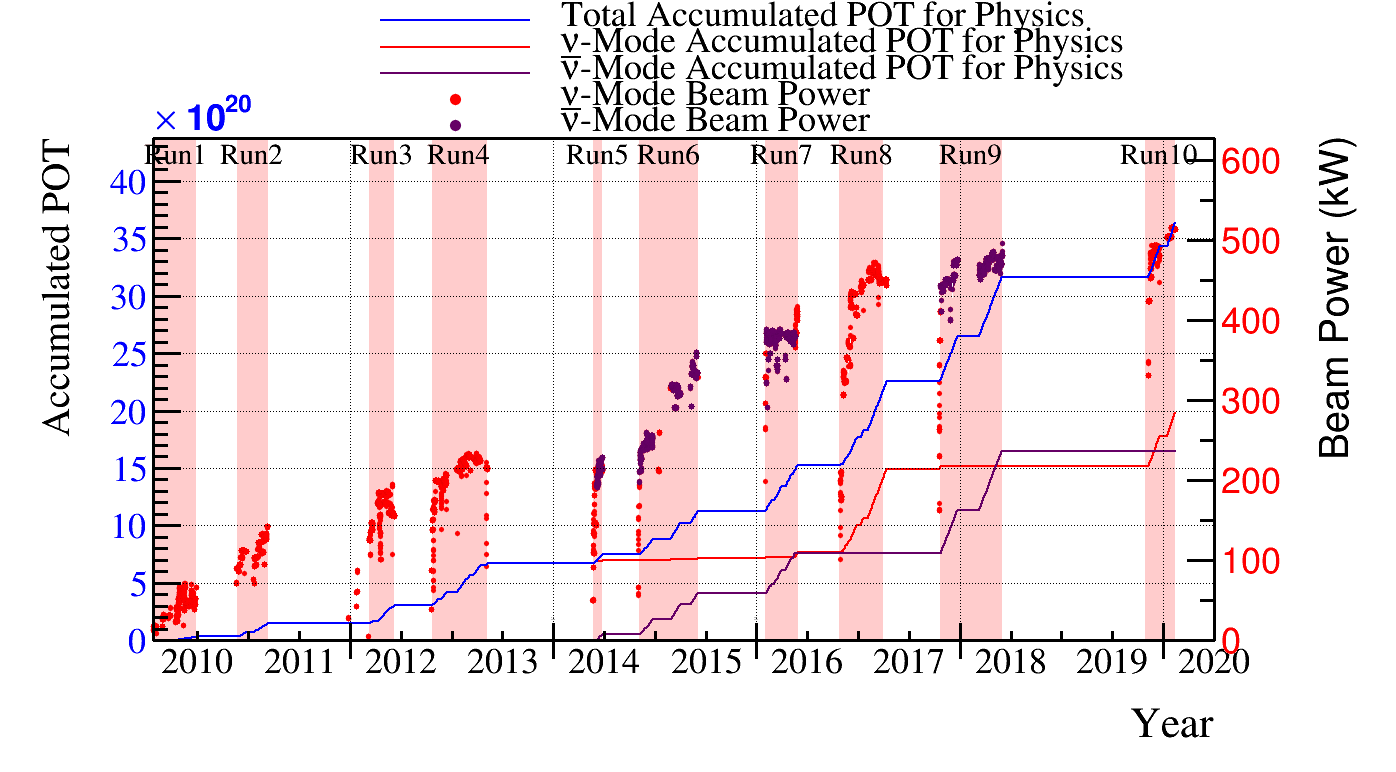
\includegraphics[width=0.7\linewidth]{POT}
  \caption{The collected statistics in the T2K experiment in POT (Proton On Target) together with the beam intensity along the data accumulation until April 2020.}
  \label{fig:t2k:POT}
\end{figure}

The initial beam is steered with the arc section made with superconducting magnets and horizontally aligned with the direction to the detectors. At this stage, the measurements of the beam parameters are performed. The beam intensity is measured with current transformers that use toroidal coils around a cylindrical ferromagnetic core. The uncertainties of the measurements are estimated at the level of 2\%. The beam position is measured with electrostatic monitors and secondary emission monitors. The first measures the beam position with the accuracy of 450 $\mu \text{m}$, while the latter measures the beam width with the precision of 200 $\mu m$. After the measurements, the beam is directed downward and focused on the carbon target.

\subsubsection{Secondary beamline}
The secondary beamline is responsible for neutrino production. The target for protons is made of a Carbon cylinder of 2.6 cm width and 91.4 cm length (1.9 interaction length). The target core heats up to 700$^\circ$C during the operation. The target is held in a titanium case for fast heat transfer to the water cooling system. The target is inserted into the first magnetic horn, so the mesons are affected by the focusing magnetic field from the moment of production.

The meson focusing system consists of three magnetic horns. The first one contains the target where the mesons are produced. The horns are operated with the pulsed current at the level of 250-320 kA. The polarity can be changed to focus negatively or positively charged mesons resulting in neutrino or anti-neutrino production. The dramatic gain of the horn usage for the neutrino beam intensity is shown in \autoref{fig:t2k:horn}.

\begin{figure}[!ht]
  \centering
    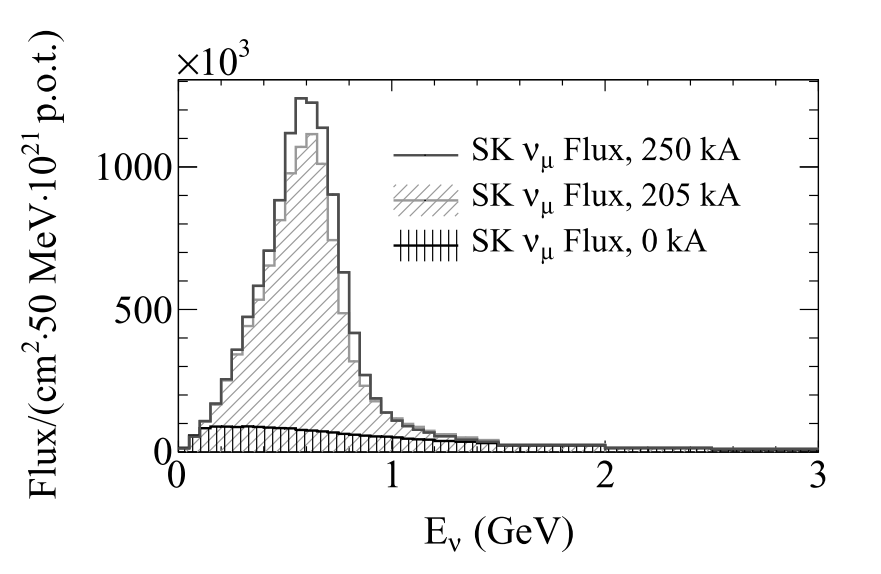
\includegraphics[width=0.5\linewidth]{horn}
    \caption{The effect of horn usage on the beam intensity at the far detector}
    \label{fig:t2k:horn}
\end{figure}

The hadrons are focused into the decay volume. It is a 96 m tunnel widening from $1.4\times1.7\text{ m}^2$ at the beginning up to the $3.0\times5.0 \text{ m}^2$ at the end. The volume is filled with Helium gas and is cooled with water. The particles possibly producing neutrinos are $\pi^\pm$, $K^\pm$, $K^0_L$ and $\mu^\pm$. The most probable neutrino production reactions are:
\begin{align}
\pi^\mp&\to\mu^\mp\overset{\scriptscriptstyle(-)}{\nu_\mu} \hspace{2cm} &K^\mp\to\mu^\mp\overset{\scriptscriptstyle(-)}{\nu_\mu} \\
K^\mp&\to\pi^0e^\mp\overset{\scriptscriptstyle(-)}{\nu_e} \hspace{2cm}  &\mu^\mp\to e^\mp\overset{\scriptscriptstyle(-)}{\nu_\mu}\overset{\scriptscriptstyle(-)}{\nu_e}
\end{align}

The energy spectra divided into neutrino flavor and parent particle are provided in \autoref{fig:t2k:nu_beam}.

\begin{figure}[!ht]
  \begin{minipage}{0.49\linewidth}
    \centering
    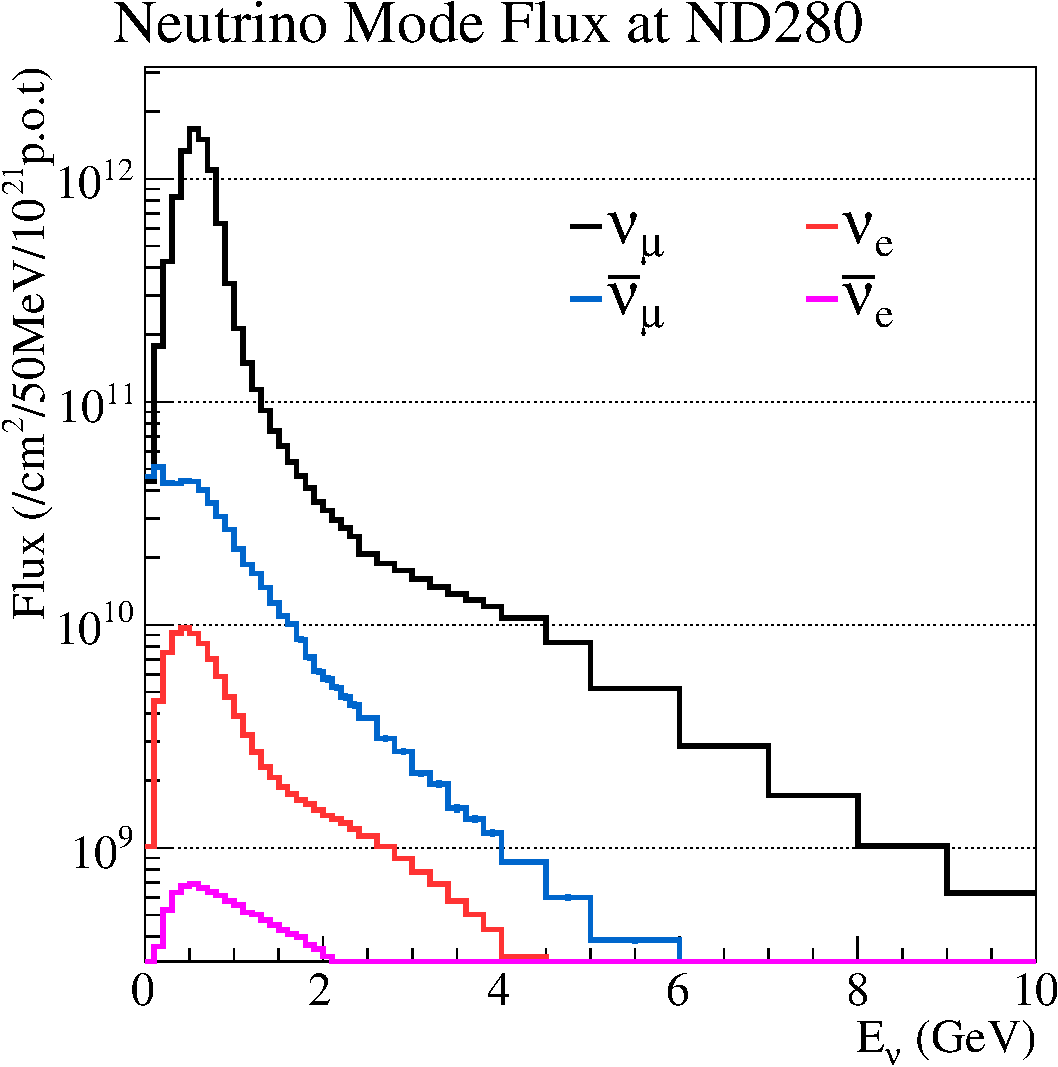
\includegraphics[width=0.5\linewidth]{nu_flux_flavor.pdf} \\ (a)
  \end{minipage}
  \begin{minipage}{0.49\linewidth}
    \centering
    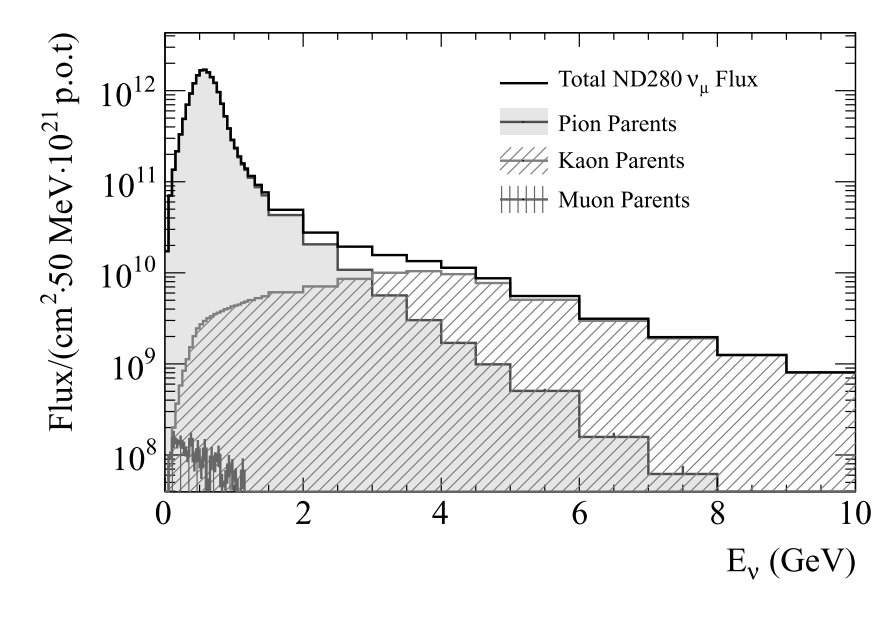
\includegraphics[width=\linewidth]{nu_flux_parent} \\ (b)
  \end{minipage}
  \caption{The neutrino beam at the near detector side divided into (a) neutrino flavor and (b) parent particle.}
  \label{fig:t2k:nu_beam}
\end{figure}

The beam dump is placed just after the decay pipe. It is made of 75 tons of graphite and suppresses all the charged particles except the high energy muons (E>5 GeV). Thus a majority of low energy muons will not decay in flight, producing electron neutrinos pointed to the far detector. It is critical for successful oscillation analysis. High energy muons can be used for the neutrino beam stability monitoring. They are mostly produced along with neutrinos in the 2-body meson decays. Thus the muon direction will explicitly indicate the direction of the neutrino beam. The muon monitor is made with an array of ionization chambers and another array of silicon PIN photodiodes. The center of the muon profile is reconstructed with 3 cm precision resulting in 0.25 mrad angular accuracy.

The overview of the T2K secondary beamline together with the near detector complex is presented in \autoref{fig:t2k:horns}.

\begin{figure}[!ht]
  \centering
  \includegraphics[width=0.9\linewidth]{horns}
  \caption{The overview of the T2K secondary beamline and the near detectors.}
  \label{fig:t2k:horns}
\end{figure}

\section{Near detector}
\label{sec:T2K:nd}
Precise knowledge about the initial neutrino beam is essential for the accurate oscillation measurements. The T2K near detector complex is placed at 280 meters from the proton target and its main goal is the monitoring of the unoscillated beam. Two detectors are used for this purpose: on-axis INGRID and off-axis ND280. The schematic views of both detectors are presented in \autoref{fig:T2K:ND280}.

\begin{figure}[!ht]
  \centering
  \begin{minipage}{0.49\linewidth}
    \centering
    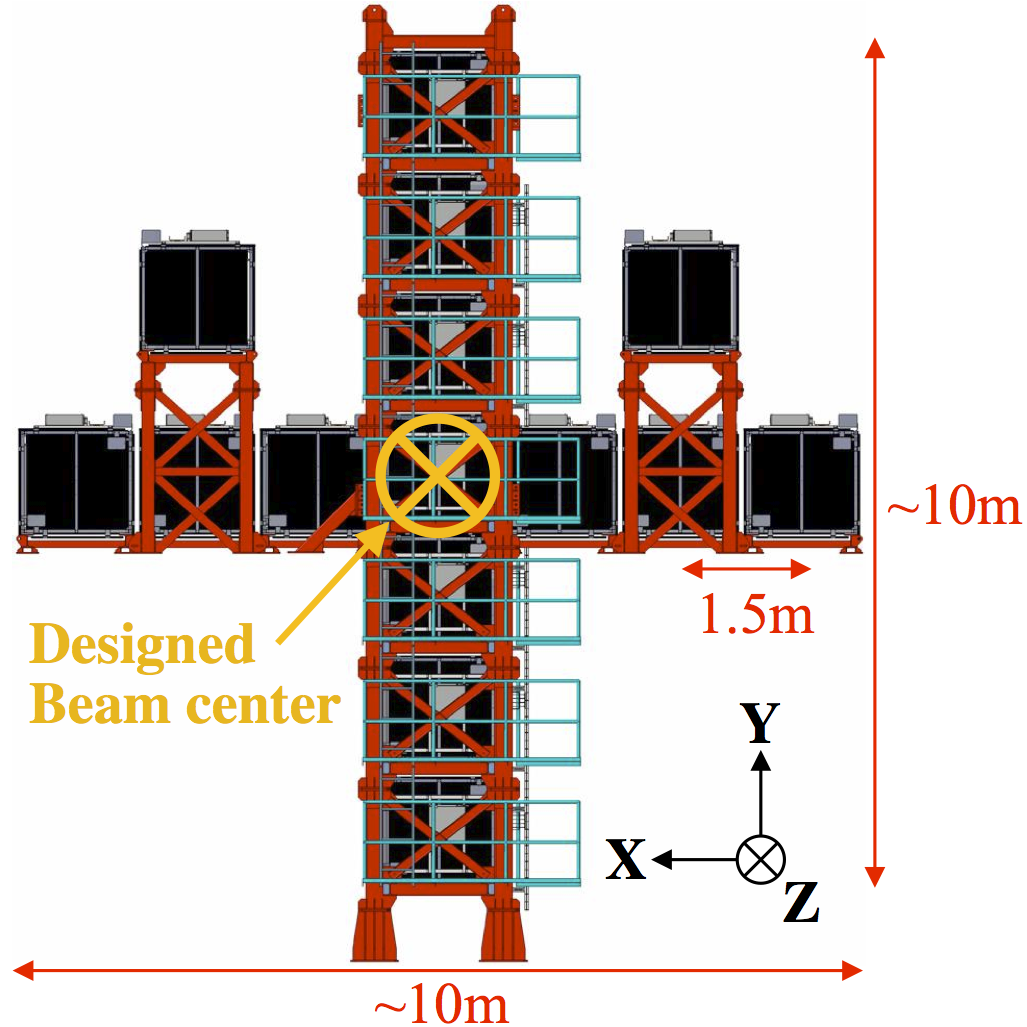
\includegraphics[width = \linewidth]{INGRID} \\ (a)
  \end{minipage}
  \begin{minipage}{0.49\linewidth}
    \centering
    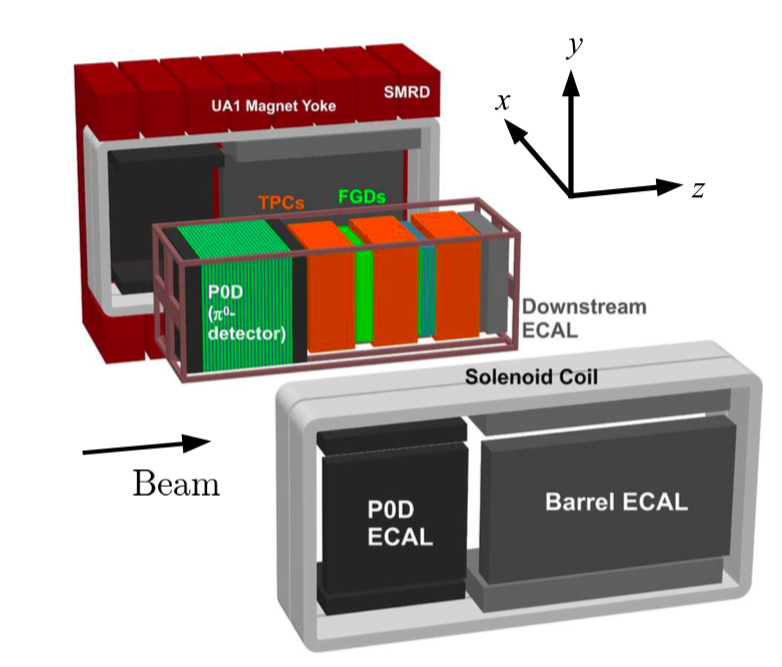
\includegraphics[width = \linewidth]{ND280} \\ (b)
  \end{minipage}
    \caption{An exploded view of the near detector complex: (a) on-axis INGRID detector, (b) off-axis ND280 detector.}
    \label{fig:T2K:ND280}
\end{figure}

\subsection{INGRID}
The main goal of the INGRID detector is controlling the position and intensity of the neutrino beam. It consists of 14 modules arranged in a cross with two additional modules placed outside the main cross (\autoref{fig:T2K:ND280} (a)). The center of the cross is placed at 0$^\circ$ angle w.r.t. proton beam direction. Each detector module consists of a sandwich of iron and tracking planes. We expect enough neutrino interactions in the iron targets every day for the day-to-day monitoring of the neutrino beam parameters: intensity and direction. \autoref{fig:t2k:ingrid_beam} represents the results of such measurements. Both intensity and direction variations are small and the related uncertainties in the oscillation analysis are negligible. The initial requirement for the beam direction accuracy was set to 1 mrad.

\begin{figure}[!ht]
  \centering
  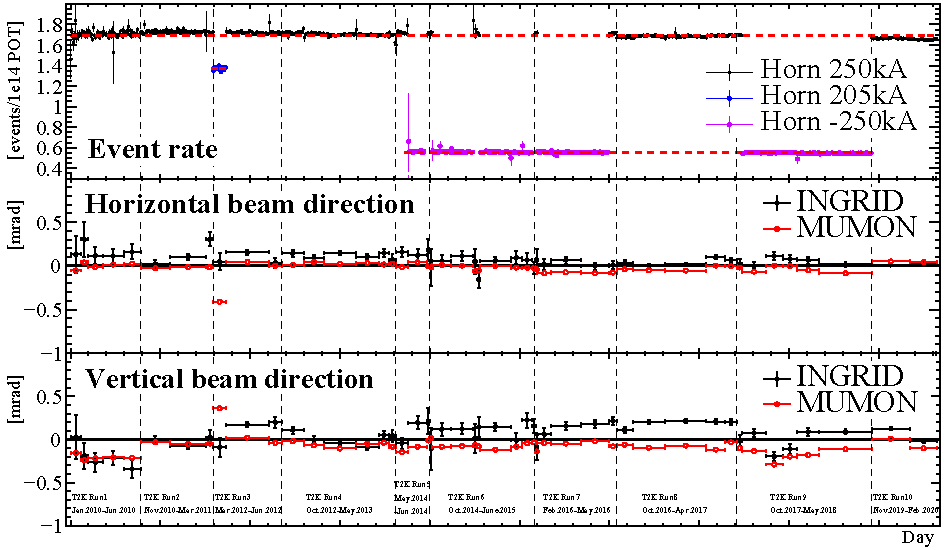
\includegraphics[width=0.8\linewidth]{ingrid_beam}
  \caption{The INGRID measurements of the neutrino beam intensity and position.}
  \label{fig:t2k:ingrid_beam}
\end{figure}

\subsection{Near detector ND280}
\label{sec:T2K:nd280}
The ND280 is an off-axis detector centered at the line from the target towards the far detector Super-Kamiokande. Its goal is measurements of the neutrino interaction dividing them into neutrino/anti--neutrino, flavor and reaction topology. The incoming neutrino energy is reconstructed from measurements of the lepton kinematics from quasi--elastic interactions. For this purpose, the detector is composed of different sub-detectors. The Fine Grained Detectors (FGD) are used as a target for neutrino interaction and the tracking of the outgoing particles. The gaseous Time Projection Chambers (TPC) are used for the charged particle tracking. The particle charge and momentum are measured with the track curvature in gas. The type of the particle is also reconstructed with the ionization energy losses. Thus the incoming neutrino type (neutrino/anti-neutrino), flavor and energy can be determined. The electromagnetic calorimeter (ECAL) detects the gamma conversion and improves electron and muon separation. The SMRD detector works as a trigger for the cosmic rays and may help with the muon identification. The P0D detector is used for the measurements of the $\pi^0$ production in the neutrino interactions.

The ND280 measurements are used to constrain the parameters of the flux and the theoretical models of the neutrino interactions. The fact that we know the neutrino type, flavor, energy and the reaction type allows us to probe several models' parameters independently. This will result in the smaller uncertainty of the global oscillation analysis. The subdetectors structure and features will be overviewed in the following subsections.

\subsubsection{$\pi^0$ detector (P0D)}
\label{sec:t2k:pod}
The primary goal of the P0D detector is to measure the cross-section of the $\pi^0$ production in the neutrino interactions through the neutral current (NC). As was mentioned in the introduction it was believed to be the main background for the $\nu_e$ appearance measurements in the far detector. The asymmetrically converted photons from the $\pi^0$ decay can be misreconstructed as $\nu_\mu\to\nu_e$ signal and bias the oscillation analysis. The same flux and the same target material should be used for accurate background treatment. As the detector is aimed to detect the NC$\pi^0$ production it should be good in the charged particle tracking to distinguish CC and NC interactions. Also, it should be effective for photon detection. The sensitive volume of the P0D is made from scintillator bars aligned along X and Y axis (perpendicular to the beam axis). The readout is done with wavelength shifting fibers (WLS). The XY scintillator layers are alternated with brass sheets and water bags. Such a structure allows efficient reconstruction of a charged particle track as well as an electromagnetic shower. The latter is used for photon detection. The scintillator layers are alternated with the lead sheets instead of water bags in the upstream and downstream parts of the detector. This improves the containment of the EM showers. The measurements of the $NC\pi^0$ production can be done with and without water in the target, thus the cross-section on water can be extracted.

\subsubsection{Fine grained detectors (FGD)}
Two FGD modules~\cite{Amaudruz2012} are used as a target for the neutrino interactions. The size of the module is $2\times2\times0.3$ $\text{m}^3$. They consist of a sandwich structure of bars made with plastic scintillators and oriented along X and Y axis, while the beam is coming along Z axis. The bars are pierced with WLS for the light collection and transportation to the photosensors. The light readout is done with multi-pixel photo counters (MPPC) that provide high detection efficiency and sufficient dynamic range.

In the second FGD the plastic layers are alternated with the water modules. Thus the measurements of the neutrino interaction with the water can be done. Such a measurement is important in the context of T2K as far detector uses water target only. The difference between neutrino interaction cross-section with Carbon and Oxygen can be a source of systematic uncertainty.

\subsubsection{Time projection chambers (TPC)}
\label{sec:t2k:tpc}
The TPCs~\cite{Abgrall2011} are gaseous detectors that perform the 3D reconstruction of the charged particle's track. The scheme of the detector is presented in \autoref{fig:t2k:tpc}.

\begin{figure}[!ht]
  \centering
  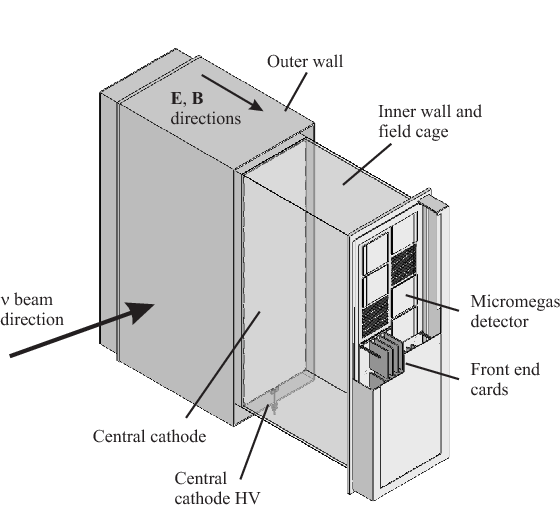
\includegraphics[width=0.6\linewidth]{tpc_module}
  \caption{The scheme of the TPC module}
  \label{fig:t2k:tpc}
\end{figure}

The general principle of the TPC operation and the key characteristics of the T2K TPCs are presented in \autoref{fig:t2k:tpc_p}. The active volume of the detector is filled with the gas mixture of Argon, $\text{CF}_4$ (tetrafluoromethane) and $\text{iC}_4\text{H}_{10}$ (isobutane) in the volume proportions 95:3:2. A charged particle going through the gas volume loses energy through ionization. The electrons from the ionization drift against the direction of the electric field --- from the cathode towards the micromegas. The positive ions are drifting towards the cathode. The Argon was chosen as a main component of the gas mixture because it is a noble gas. It is very easy to ionize thus we will have a lot of initial electrons. Also, it will not subject to a chemical reaction. It is especially important in the amplification region, where chemical reactions are most probable. Isobutane provides quenching of the avalanche in the amplification region by absorbing UV photons. $\text{CF}_4$ is responsible for the speed-up of the electron drift. Such a mixture is very powerful resulting in high speed, low diffusion, and good performance with micromegas detectors.

\begin{figure}[!ht]
  \centering
  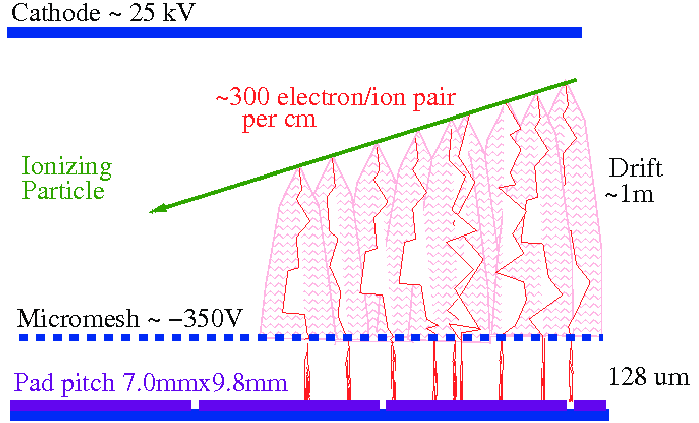
\includegraphics[width=0.5\linewidth]{TPC_principe}
  \caption{The general concept of the TPC operation.}
  \label{fig:t2k:tpc_p}
\end{figure}

The electric field strength is constant in the drift region. The voltage between the cathode and micro mesh is 25 kV at a distance of ~1 meter. The signal is dramatically amplified between the micro mesh and pads as a voltage of 350 V is applied to the 128 $\mu \text{m}$ gap. The produced avalanches are detected with the $6.9\times9.7$ $\text{mm}^2$ pads. Here the electrons avalanche produce the analog electric signal that will be later digitized with the electronics.

In total, the readout surface of one TPC module consists of 12 micromegas $48\times36$ pads each. The 2D projection (YZ) of the track is reconstructed with the hit pads. The drift time is measured to reconstruct the track curvature in XY plane. The external detector (FGD) is used for the reconstruction of the absolute position along X axis.

The core of the ND280 --- the tracker, consists of 3 TPCs alternated with 2 FGDs. Such a structure is aimed at the effective detection of the lepton produced in the neutrino interactions inside FGDs. The particle type, sign and momentum can be precisely measured with such a setup.

The particle type is estimated based on its ionization loss. The mean deposited energy  for the particular particle with given momentum is described with Bethe--Bloch formula~\cite{Bethe1930}. But the fluctuations follow Landau distribution~\cite{Landau1944} and are rather large. The distributions of the energy loss per unit length for the particles from neutrino interactions in ND280 are shown in \autoref{fig:t2k:tpc_dedx}. Four hypotheses for the particle type are considered: electron, muon, pion, and proton. For each hypothesis, the expected energy loss is compared with the measured values. The cut on the likelihood value is set to find out if the given track satisfies the hypothesis of the particular particle type.

\begin{figure}[!ht]
  \centering
  \begin{minipage}{0.49\linewidth}
    \centering
    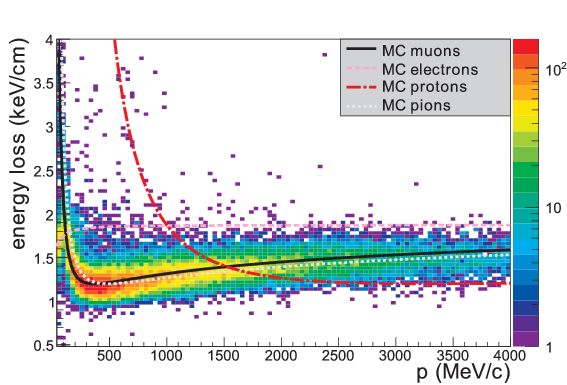
\includegraphics[width=\linewidth]{tpc_neg} \\ (a)
  \end{minipage}
  \begin{minipage}{0.49\linewidth}
    \centering
    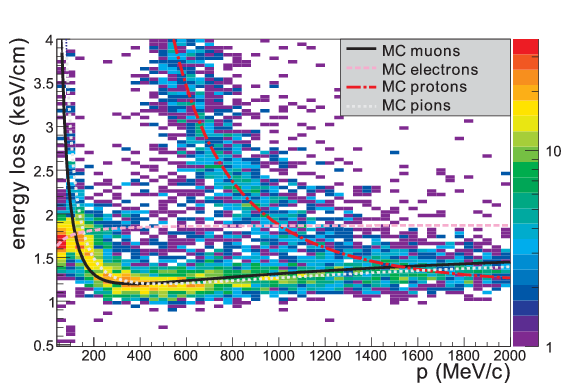
\includegraphics[width=\linewidth]{tpc_pos} \\ (b)
  \end{minipage}
  \caption{The distribution of the energy loss per unit length for the (a) negatively and (b) positively charged particles produced in neutrino interactions in ND280 TPCs}
  \label{fig:t2k:tpc_dedx}
\end{figure}

\subsubsection{Electromagnetic calorimeter (ECaL)}
The calorimeters are used for the detection of the gammas from the $\pi^0$, produced in the neutrino interactions. They also can help with particle identification. Electrons and hadrons will produce showers while muons will have a clear clean track. The calorimeters are surrounding the inner detectors of the ND280. They consist of the sandwich structure of plastic bars $4\times1$ $\text{cm}^2$ in cross-section, alternating with 1.75 mm thick absorber layers made with lead. The downstream ECaL consists of 34 layers and provides the most precise results, while P0D and barrel ECaL consists of 31 layers.

\subsubsection{Side muon range detector (SMRD)}
The SMRD is surrounding the whole ND280 and is a multifunction detector. It allows rejecting the events triggered by the cosmic rays or the neutrino interactions in the outer detectors or concrete of the pit. SMRD is useful for the detection of the muons that exit the detector with high angles. Since there is no TPC in this direction the momentum measurement can be done only with SMRD. The detector itself consists of 440 1.7 cm thick plastic scintillator modules that are inserted in the gaps between 4.8 cm thick steel plates of the magnet yoke.


\section{Super--Kamiokande}
\label{sec:T2K:sk}
The far detector of the T2K experiment is Super--Kamiokande (SK)~\cite{Fukuda2003} located 295 km away from the proton target in the Kamioka mine. 50 tons of water is used as a target for neutrino interactions. The water tank is viewed by 13 thousand photomultipliers (PMT) aimed at the detection of Cherenkov light from the charged lepton produced in the neutrino interactions. The schematic view of the detector is presented in \autoref{fig:t2k:sk}.

\begin{figure}[!ht]
  \centering
  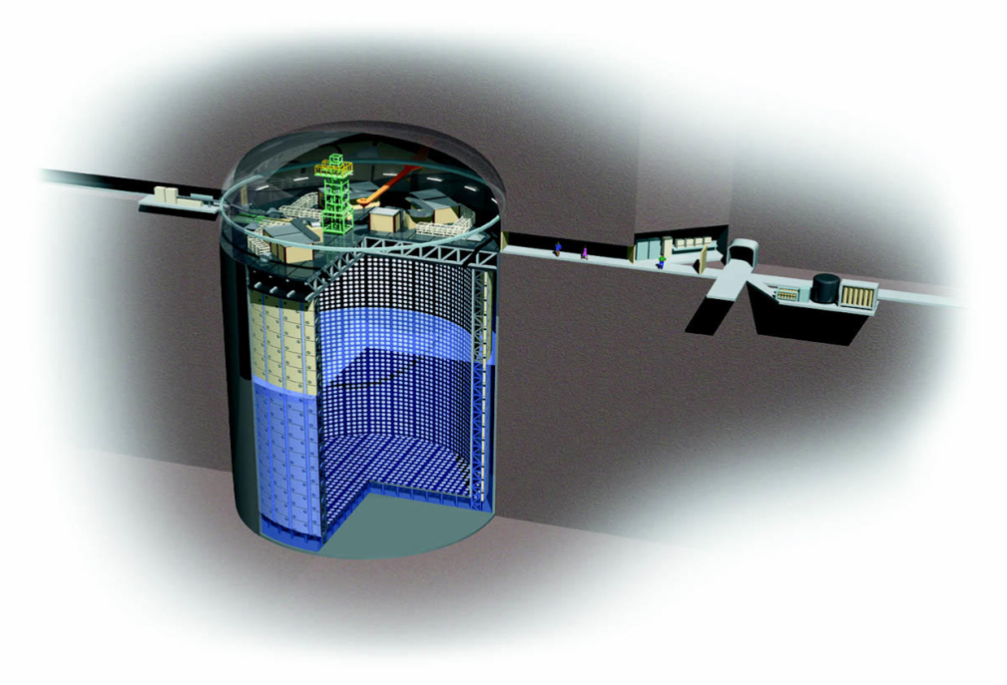
\includegraphics[width=0.7\linewidth]{sk_tank}
  \caption{The scheme of the Super-Kamiokande detector.}
  \label{fig:t2k:sk}
\end{figure}

The working principle of the detector is based on the effect of Cherenkov radiation. When a charged particle passes through a dielectric medium at a speed greater than the phase velocity of light in that medium a conic wavefront is formed. The opening angle of the cone is defined by the particle speed and the refraction index of the medium $\cos{\theta}=1/n\beta$, where $\beta=v/c$. The emission of the radiation is a threshold effect. As could be seen from the equation above, the wavefront can be formed only if the particle is fast enough $\beta>1/n$. For the water detector, the thresholds are 1.4 GeV for protons, 160 MeV for muons and 775 keV for electrons. The maximum angle is also limited by $\theta_{max}=\arccos(1/n)\approx42^\circ$.

Super-Kamiokande continues the successful history of the neutrino detectors in the Kamioka mine. The first experiment KamiokaNDE (Kamioka Nucleon Decay experiment) started looking for the nucleon decays in 1983. The atmospheric neutrino interactions were the main background. During the detector operation, a nice performance of the neutrino detection was observed and the experiment was refocused on the neutrino analysis. Since then the detector was massively improved and new setups were built: Kamiokande II, Super-Kamiokande. The latter is operating now as a far detector of the T2K experiment. The experience collected during the studies in Kamioka allows excellent physics performance.

There are many challenges in neutrino studies with water Cherenkov detectors. First of all, the statistics is limited due to the small cross-section. To increase the number of events the detector was enlarged several times from 3 kt (KamiokaNDE) to 50 kt (Super-Kamiokande). But the detection of Cherenkov light becomes an issue with a larger tank. The intensity of such a light is quite low. Thanks to the hard work of the SK collaboration the water purity is extremely high. The transparency is very stable at the level of 100 meters. The other issue is the photon detection itself. The photo coverage of the active area surface is 40\% aiming at the collection as many photons as possible. Large 20-inch PMTs with high detection efficiency are used for it. The wavelength of Cherenkov light extends to the ultraviolet region, while the efficiency of the PMTs is quite low there. The light intensity decreases as $\lambda^3$ with the increasing of the wavelength, that's why the excellent performance of the PMT is essential for the successful detector operation.

The other challenge is background suppression. The detector is placed in a mine to reduce the flux of the cosmic rays. However, extremely high energy muons can reach the water tank. Also, muons can be produced by the neutrino interactions in the rock close to the detector. The Super--Kamiokande is divided into two volumes: inner and outer detectors. They are optically isolated, so a signal detection in the outer volume will explicitly indicate an out-of-tank particle production. Only leptons produced in the inner detector are considered for the neutrino analysis.

The detector allows separating Cherenkov ring produced by muon and electron. Due to their lighter mass electrons are more subject to bremsstrahlung. Since the critical energy for the electrons in water is tens of MeV and the typical energy of the electrons produced by the T2K neutrinos is hundreds of MeV, we expect to see electromagnetic showers that will distort Cherenkov ring. The examples of the events are presented in \autoref{fig:T2K:sk_PID}. The left image demonstrated a much less distorted ring from the muon while the right image demonstrates the result of the electron showering. Up to now, the Super--Kamiokande separates these two topologies with excellent purity. The probability to identify a single electron (muon) as muon (electron) is 0.7\% (0.8\%). That's extremely important for the oscillation experiment. The neutrino will produce the charged lepton of the same flavor and we are studying a very rare process of the electron neutrino appearance. That's why any confusion between muon and electron is extremely dangerous.

\begin{figure}[!ht]
  \centering
  \begin{minipage}{0.49\linewidth}
    \centering
    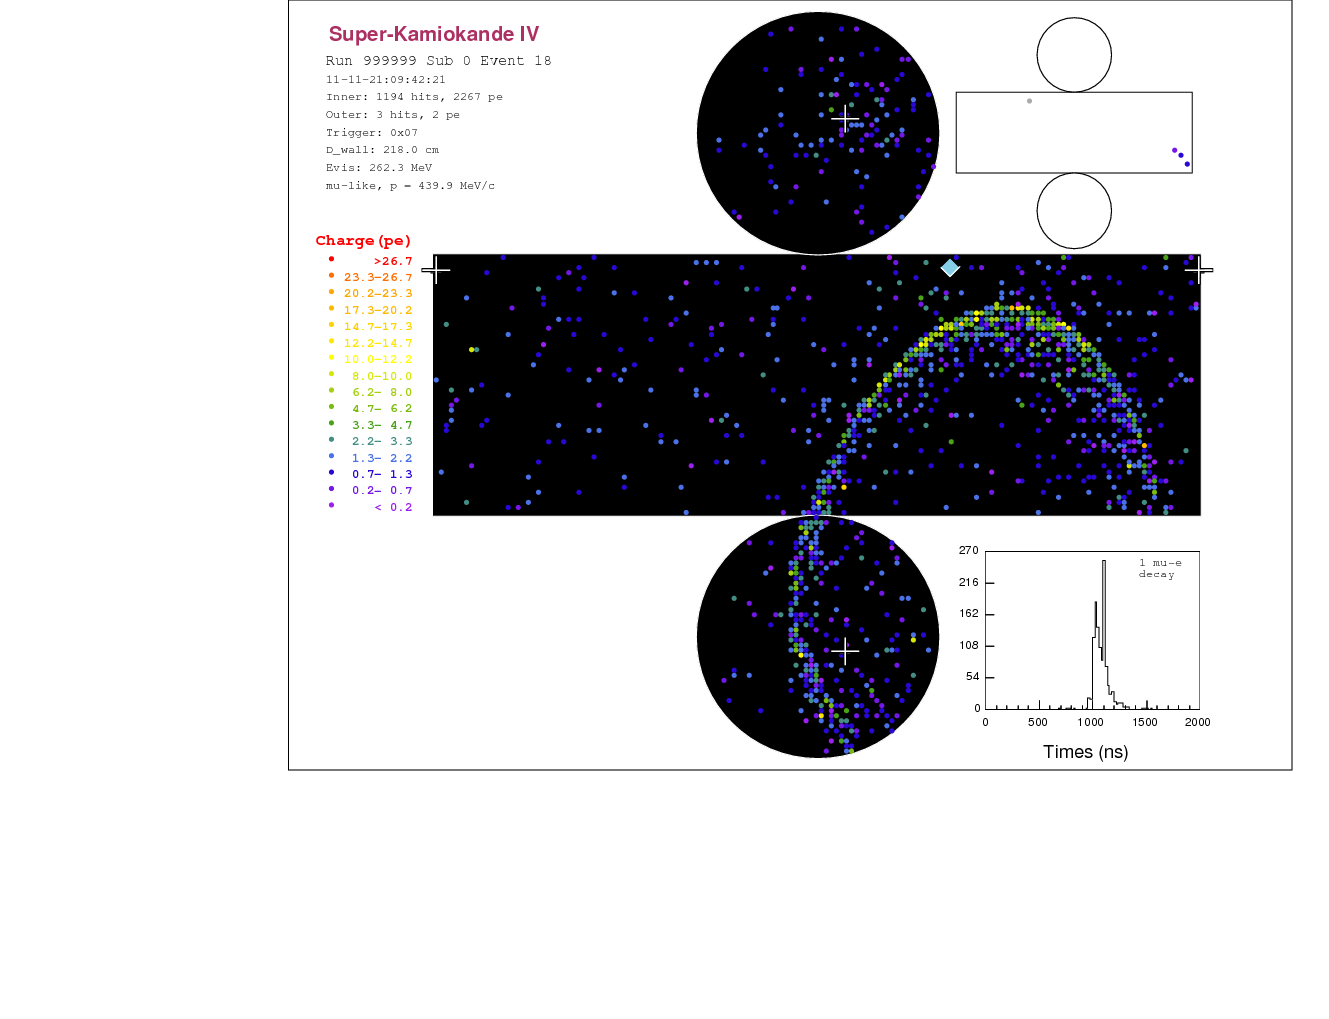
\includegraphics[width = \linewidth]{sk_mu} \\ (a)
  \end{minipage}
  \begin{minipage}{0.49\linewidth}
    \centering
    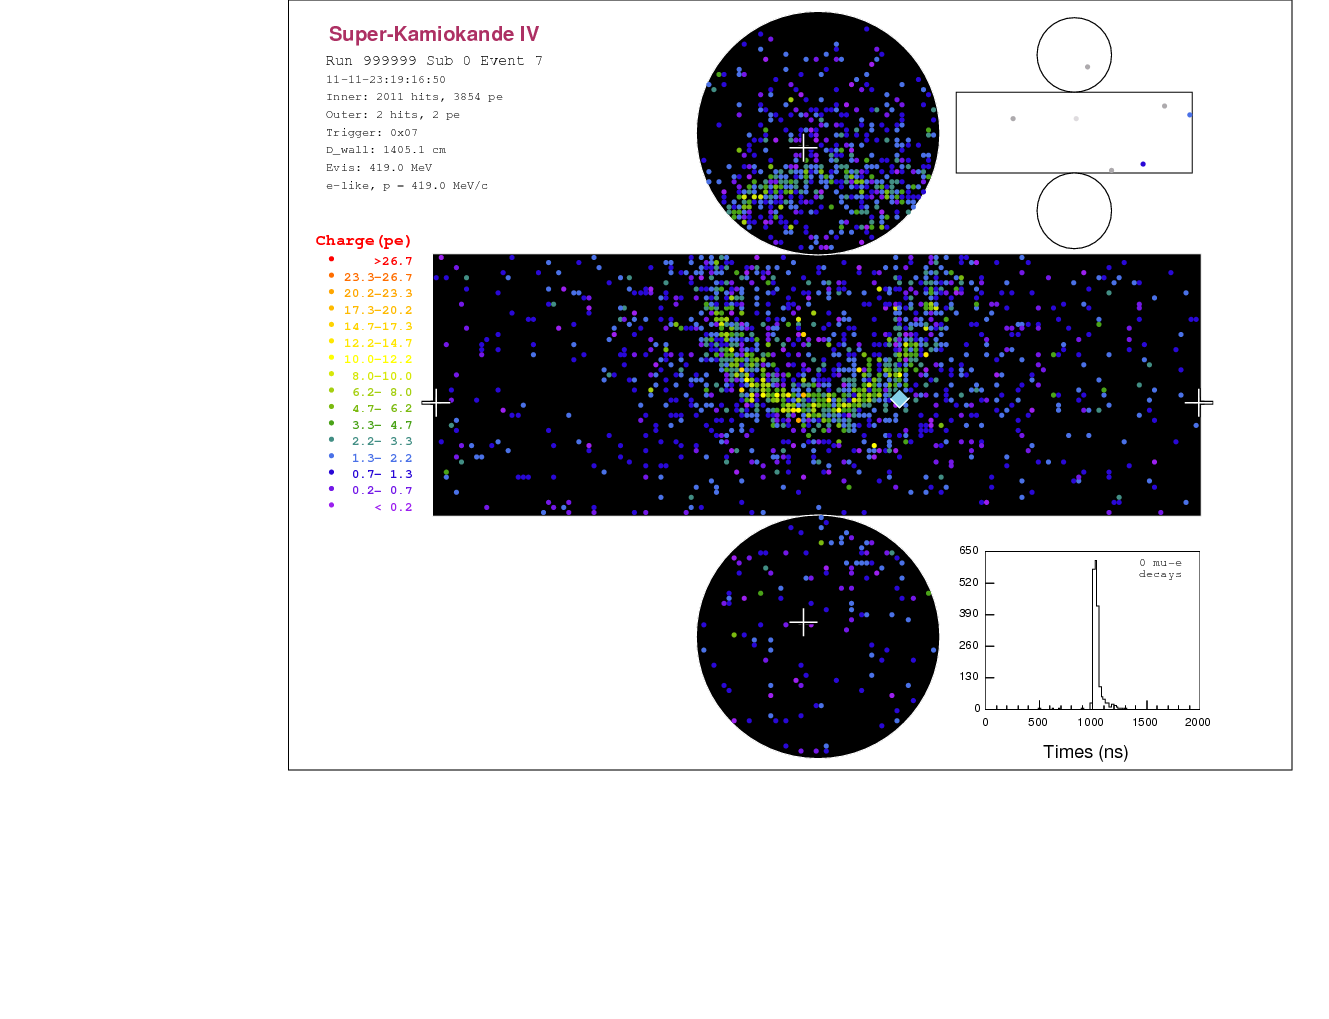
\includegraphics[width = \linewidth]{sk_e} \\ (b)
  \end{minipage}
    \caption{The event display of Cherenkov ring inside Super-Kamiokande detector: (a) ring from muon, (b) ring from electron.}
    \label{fig:T2K:sk_PID}
\end{figure}

The Super--Kamiokande provides powerful shielding from the cosmic rays, but the atmospheric neutrino can easily go through the rock and interact inside the inner detector. That's how the atmospheric studies are done, but for the T2K we need to distinguish neutrinos from the atmosphere and J-PARC accelerator. For this purpose, the timing information is the most useful one. As mentioned in \autoref{ch:T2K:nu_beam} the beam is grouped in 8 bunches 19 ns width coming every 2 seconds. The time synchronization between J-PARC and Super-Kamiokande allows us to select accurately neutrinos that fall into bunches and suppress the atmospheric background that is uniform in time. Thus the background is suppressed by 8 orders of magnitude.


\section{Analysis overview}
\subsection{Oscillation analysis}
\subsubsection{General overview}
As mentioned in the introduction the main goal of the T2K experiment is precise measurements of the neutrino oscillation parameters and search for the CP--violation in the lepton sector. This is done by measuring the neutrino energy spectrum at the far detector and comparing it with the expectation without the oscillations. Spectra are divided into the neutrino flavor (muon and electron) and type (neutrino/anti--neutrino), thus 4 spectra are the basic input for the oscillation analysis. Super--Kamiokande measures neutrino energy with the assumption of the quasi--elastic interaction (\autoref{eq:t2k:sk_e}).

\begin{equation}
\label{eq:t2k:sk_e}
E_\nu^{rec}=\frac{m_f^2-(m_i')^2-m_\ell^2+2m_iE_\ell}{2\left(m_i'-E_\ell+p_\ell\cos\theta_\ell\right)}
\end{equation}
where $E_b = 27\text{ MeV}$ is called ``liberation\footnote{Sometimes notated as a ``binding''} energy'' and it is mean energy that is required to eject a nucleon from the Oxygen nucleus, $m_i'=m_i-E_b$, $m_i$ and $m_f$ are initial and final nuclei mass respectively, $m_\ell$, $E_\ell$, $p_\ell$, $\theta_\ell$ are outgoing lepton mass, energy, momentum and angle w.r.t neutrino beam respectively.

Four neutrino energy spectra are essential for the minimal oscillation analysis, but the precision can be dramatically improved with the near detector. ND280 is used for the constraints of the flux and cross-section models.

Despite neutrino production is well controlled the resulting flux can be slightly different from the expectations. The possible reasons are wrong assumptions about the hadron production model, proton beam profile, off-axis angle, horn current, horn alignment, and other factors. The hadron production model is responsible for the total number and spectra of the produced mesons. The horn configuration affects the meson focusing, thus can affect the intensity, symmetry and direction of the beam. Different beam off-axis angle can change the neutrino energy spectrum in our detectors. The ND280 can constrain exactly the same off-axis flux that will pass through Super--Kamiokande but before the oscillations. For each source of error mentioned above, the underlying parameters in the model are varied to evaluate the effect on the flux prediction in bins of neutrino energy for each neutrino flavor. The example of the prior and ND280 constrains on the $\nu_\mu$ flux are presented in \autoref{fig:T2K:banff} (a).

\begin{figure}[!ht]
  \centering
  \begin{minipage}{0.49\linewidth}
    \centering
    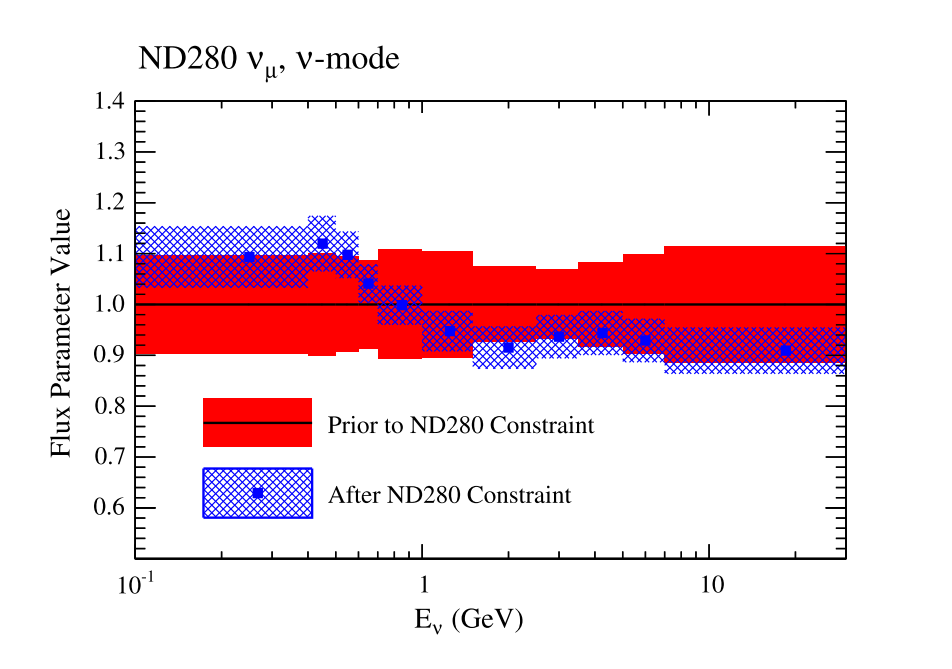
\includegraphics[width = \linewidth]{banff_flux} \\ (a)
  \end{minipage}
  \begin{minipage}{0.49\linewidth}
    \centering
    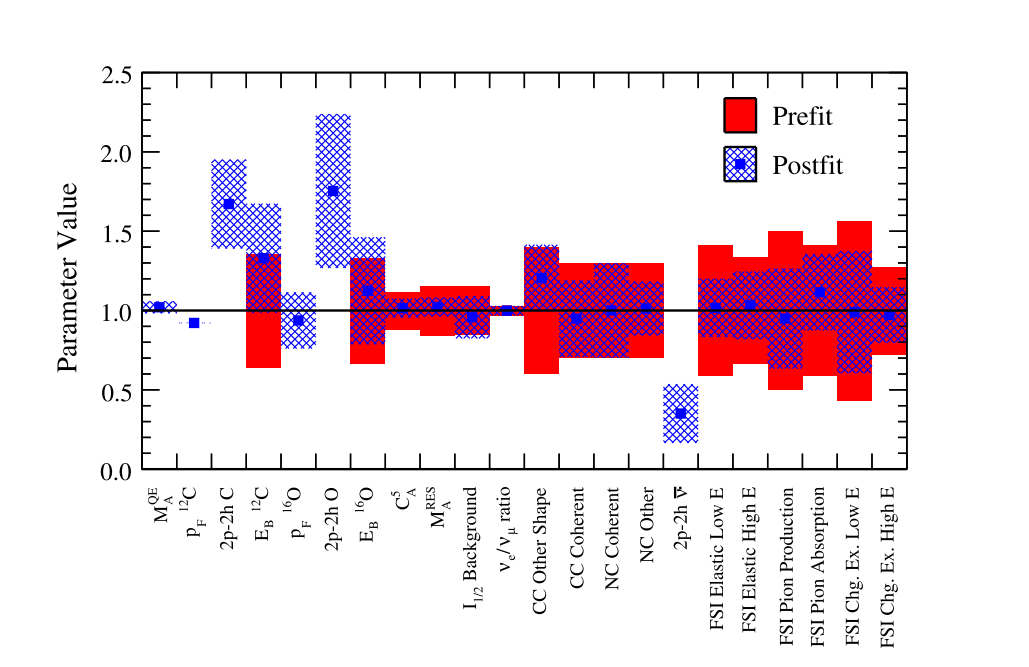
\includegraphics[width = \linewidth]{banff_xsec} \\ (b)
  \end{minipage}
    \caption{The priors (red) and the results of the ND280 fit (blue) for $\nu_\mu$ (a) flux and (b) cross-section parameters. The T2K is operating in neutrino mode. Figure from~\cite{Abe2017}.}
    \label{fig:T2K:banff}
\end{figure}

The neutrino interaction models are also tuned with the ND280 data. The models depend on many parameters. The advantage of the ND280 is the sampling of the measurements in the neutrino type, flavor and topology. ``Topology'' can be described as a multiplicity of the neutrino interaction. In ND280 we select the following topologies: CC interactions with no pions ($CC0\pi$), interactions with 1 pion ($CC1\pi$) and other CC ($CCOther$). The ``topology'' can be different from the initial reaction type because of nuclear effects (\autoref{sec:intro:nuclei} of \autoref{ch:nu_phys}). For example, after the interaction with pion production $\nu_\mu+p\to\mu^-+p+\pi^+$ the latter can be absorbed by the nucleus and the event will look exactly like quasi-elastic scattering. That is why the events are classified with the particles in the final state, but not with the type of the initial neutrino interaction. The nuclear effects add additional uncertainty in the oscillation analysis. The different model parameters are affecting different topologies. Therefore measurements with three samples will allow to precisely constrain different neutrino interaction types.

Only quasi--elastic (QE) interactions are used in the far detector for the oscillation analysis. But as was overviewed some nonQE reactions can mimic the signal. The ND280 measures both QE and nonQE interactions precisely (e.g. \autoref{fig:T2K:nd_obs}) and constrain the models parameters that affect particular reactions (\autoref{fig:T2K:banff} (b)). Thus this type of background is constrained.

\begin{figure}[!ht]
  \centering
  \begin{minipage}{0.49\linewidth}
    \centering
    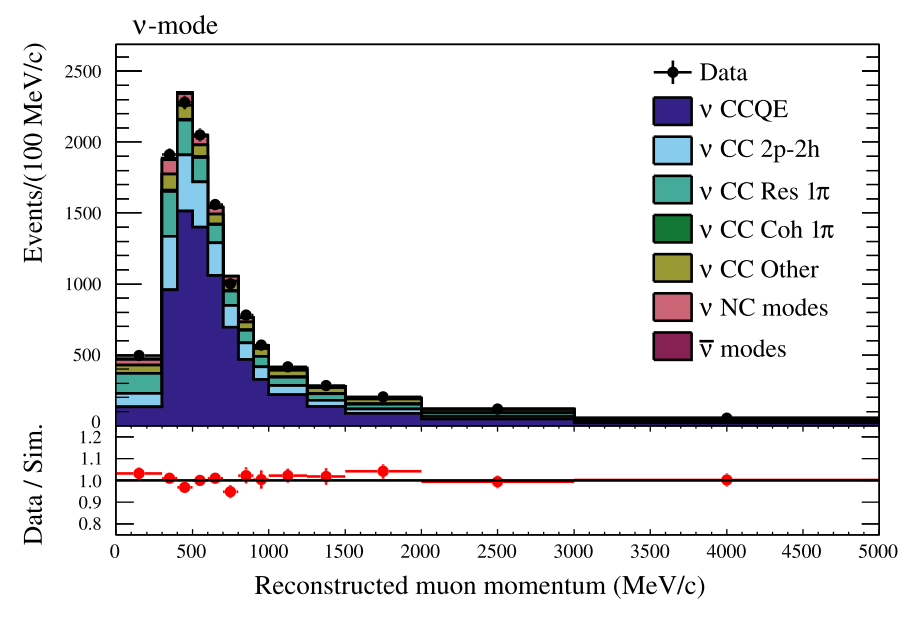
\includegraphics[width = \linewidth]{nd280_0pi} \\ (a)
  \end{minipage}
  \begin{minipage}{0.49\linewidth}
    \centering
    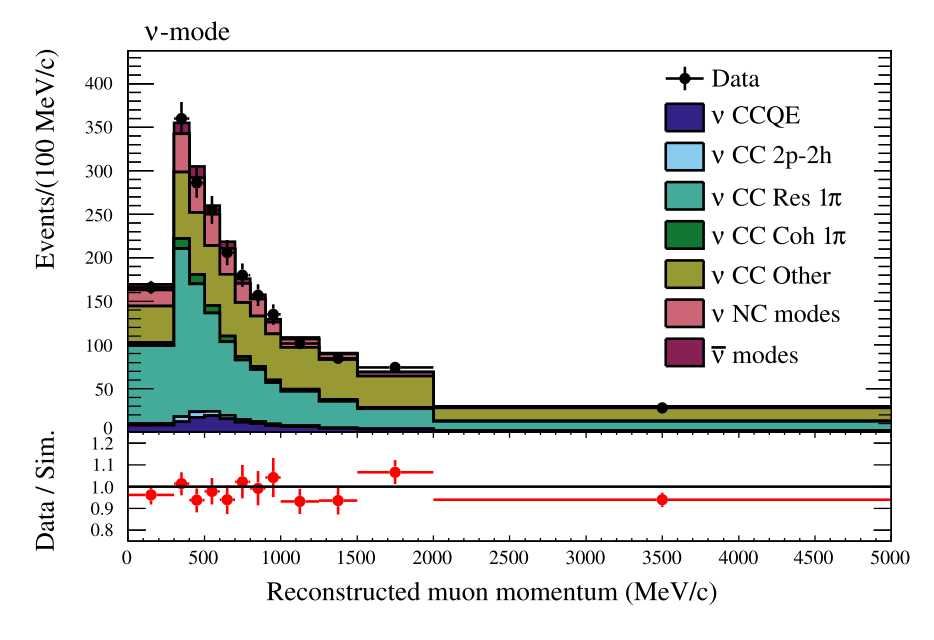
\includegraphics[width = \linewidth]{nd280_1pi} \\ (b)
  \end{minipage}
    \caption{Data MC comparison for the (a) $CC0\pi$ and (b) $CC1\pi$ samples measured with the ND280 in the neutrino mode. Figure from~\cite{Abe2017}.}
    \label{fig:T2K:nd_obs}
\end{figure}

\subsubsection{Analysis machinery}
The scheme of the analysis workflow is presented in \autoref{fig:t2k:ana}. Different colors at the block-scheme represent the measurements (green), models (violet) and fit algorithms (blue).

\begin{figure}[!ht]
  \centering
  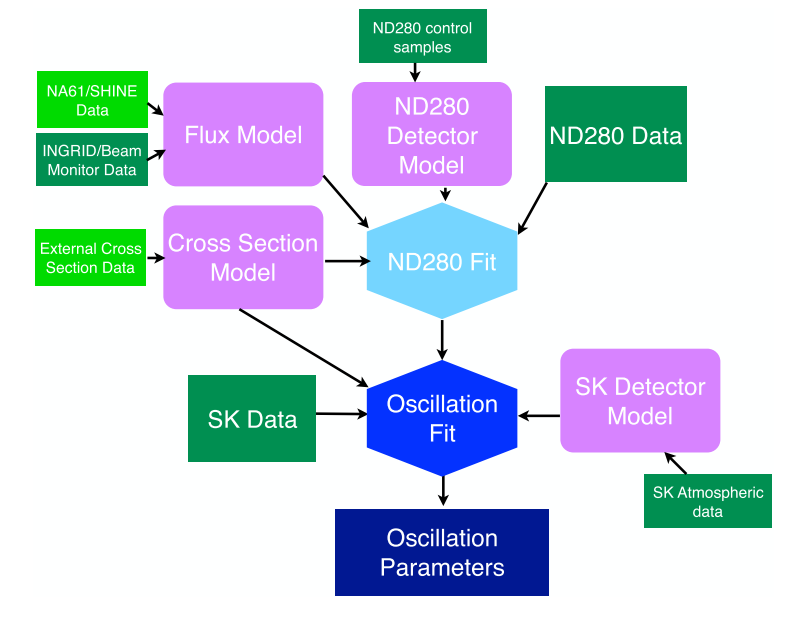
\includegraphics[width=0.8\linewidth]{t2k_ana_scheme}
  \caption{The scheme of the T2K oscillation analysis workflow. The measurements are presented in green (light --- external, dark --- T2K), the models are presented in violet and the fitter tools are presented in blue.}
  \label{fig:t2k:ana}
\end{figure}

The measurements start with the beamline monitors where the parameters of the proton beam are estimated. Then the data from the NA61 experiment is used to estimate the meson production in the target. The neutrino beam intensity and direction are monitored with the on-axis near detector INGRID. All these results allow us to build the neutrino flux model.

The near detector ND280 performs the measurements of the neutrino interaction rate. The observations are sampled in the neutrino/anti--neutrino interactions and the reaction topology: quasi-elastic, pion production, deep inelastic. We use the results of other experiments as a prior estimation for the cross-section of neutrino interactions. But there are several parameters in the model that can be tuned precisely using all the samples collected in the ND280. Thus flux and the cross-section model are tuned together with the ND280 control samples.

The long history of the atmospheric neutrino measurements in Super-Kamiokande provides accurate knowledge of the detector operation. This detector response model is used together with the T2K events in the SK for the final oscillation measurements. The spectrum of the observed electron neutrinos in the far detector are compared to the expectations without the oscillations is presented in \autoref{fig:t2k:nu_e}.

\begin{figure}[!ht]
  \centering
  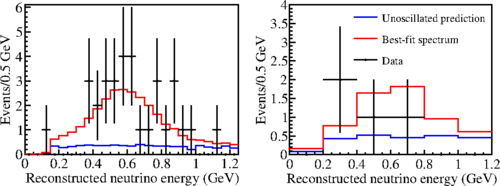
\includegraphics[width=0.9\linewidth]{nu_e}
  \caption{The spectrum of the electron neutrinos observed in the far detector comparing to the expectations without oscillation (blue) and the best oscillation fit (red).}
  \label{fig:t2k:nu_e}
\end{figure}

As one could see the oscillation fit is the heart of the analysis. Its goal is to extract the neutrino oscillation parameters from the data sets and to estimate the impact of all the uncertainties on the final result. The likelihood minimization method is used for this purpose. The expected number of events in the far detector is assumed to follow Poisson distribution. The data is sampled in the energy bins. Therefore the likelihood function is defined with:
\begin{equation}
-2\ln\mathcal{L}\left(\overrightarrow{o}, \overrightarrow{f}\right)=2\sum^{N-1}_{i=0}\left[n_i^{obs}\cdot\ln\left(n_i^{obs}/n_i^{exp}\right)+\left(n_i^{exp}-n_i^{obs}\right)\right]
\end{equation}

The vectors $\overrightarrow{o}$ and $\overrightarrow{f}$ are neutrino oscillation parameters (the goal of the fit) and nuisance parameters respectively; $n_i^{obs}$ and $n_i^{exp}$ are observed and expected events in the i-th energy bin. The likelihood function defined above is high dimensional. The nuisance parameters can be marginalized with integration over the product of the likelihood function and priors:

\begin{equation}
\mathcal{L}_{marg}\left(\overrightarrow{o}; x\right)=\int_F\mathcal{L}\left(\overrightarrow{o},\overrightarrow{f};x\right)\pi(\overrightarrow{f})d\overrightarrow{f}=\frac{1}{n}\sum_{i=1}^{n}\mathcal{L}\left(\overrightarrow{o}; \overrightarrow{f_i}, x\right)
\label{eq:T2K:marg}
\end{equation}

This defines a function that depends only on the oscillation parameters and given data. The model parameters such as cross-section, flux, detector performance are embedded in the function as priors following Gaussian distribution. After the likelihood minimization, limits in the oscillation parameters space are set~\cite{Cousins1992}.

T2K performs three different analyses with slightly different techniques. The main strategy of likelihood minimization is the same for all of them. Two of the methods are doing it with the frequentist framework. The \autoref{eq:T2K:marg} converges to the $\chi^2$ distribution. The confidence region can be set with $-2\Delta\mathcal{L}(\overrightarrow{o})\leqslant X_{crit}(\overrightarrow{o})$. And the critical values of $X$ are taken based on the desired confidence, e.g. 90\%. The only difference between the two frequentist methods is data sampling. One of them uses outgoing charged lepton momentum with the lepton direction w.r.t. neutrino beam. The other uses neutrino energy instead of lepton momentum. Both methods are expected to give the same results and are used for the cross-check. The third analysis is using Markov chain Monte Carlo method for the likelihood minimization.

The result is considered as robust only if all the methods are in a good agreement about the confidence/credible intervals. The oscillation results are presented in \autoref{fig:T2K:osc_res}.

\begin{figure}[!ht]
  \centering
  \begin{minipage}{0.49\linewidth}
    \centering
    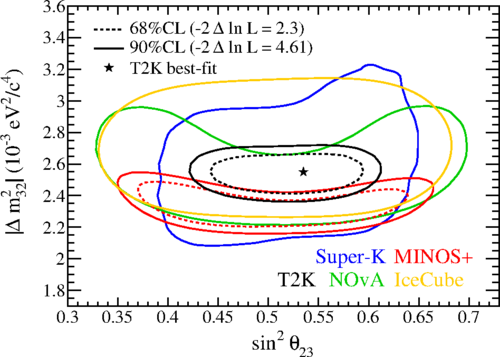
\includegraphics[width = \linewidth]{osc_res} \\ (a)
  \end{minipage}
  \begin{minipage}{0.49\linewidth}
    \centering
    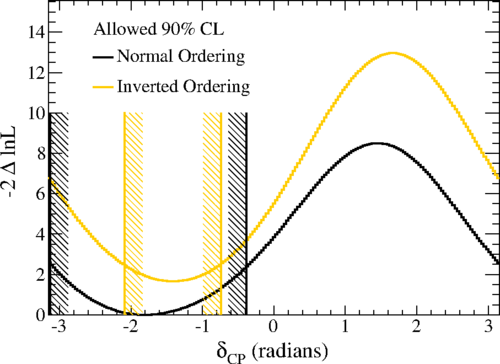
\includegraphics[width = \linewidth]{cp} \\ (b)
  \end{minipage}
    \caption{The oscillation results from the T2K experiment obtained with frequentist approach: (a) $\theta_{23}$ and $\Delta m_{32}^2$ constraints and (b) $\delta_{CP}$ constraints with statistics $3.12\times10^21$ POT}
    \label{fig:T2K:osc_res}
\end{figure}

\subsection{Neutrino cross-section measurements}
Alongside the oscillation analysis, T2K performs very precise measurements of the neutrino cross-sections. The knowledge of the neutrino interactions' rates is essential for the oscillation analysis as the most realistic theoretical model can be chosen. The ND280 provides an opportunity to study neutrino interaction with carbon, oxygen and iron with both neutrino and anti-neutrino and with both flavors: muon and electron. The dominating reaction final state in the ND280 is a muon with no pions. It is the main process for the T2K energies that's why it is studied quite well~\cite{Abe2020a}. It is more difficult to study the interaction of the electron neutrinos. The result of the comparison of the $\nu_e$ and $\overline{\nu}_e$ cross-section is presented in \autoref{fig:t2k:nue_Xsec}~\cite{Abe2020}.

\begin{figure}[!ht]
  \centering
  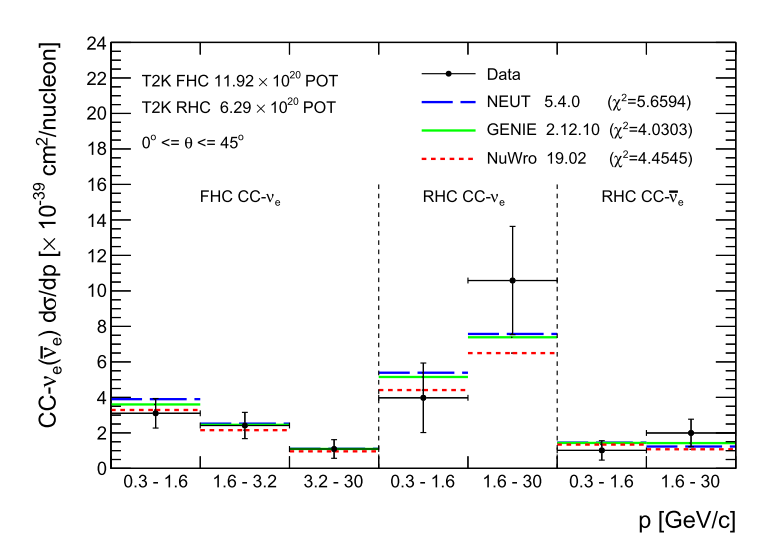
\includegraphics[width = 0.7\linewidth]{nue_Xsec}
  \caption{The result of the cross-section measurements in the ND280. Results for $\nu_e$ (Forward Horn Current, FHC) and $\overline{\nu}_e$ (Reverse Horn Current, RHC) are compared against various theoretical models.}
  \label{fig:t2k:nue_Xsec}
\end{figure}

\end{document}